\documentclass[a4paper,11pt]{article}

\usepackage{indentfirst}
\usepackage{graphicx}
\usepackage{subcaption}
\usepackage{float}
\usepackage{chngcntr,tocloft}
\usepackage{listings}
\usepackage{comment}
\usepackage{fancyhdr}
\usepackage[utf8]{inputenc}
\usepackage{indentfirst}
\usepackage{amsmath}
\usepackage{textgreek}
\usepackage{fixltx2e}
\usepackage{color}
\graphicspath{ {images/} }
\usepackage{hyperref}
\hypersetup{
    colorlinks=false,
    linkcolor=blue,
    filecolor=magenta,      
    urlcolor=cyan,
    }
\definecolor{green}{rgb}{0,0.6,0}
\definecolor{gray}{rgb}{0.5,0.5,0.5}
\definecolor{mauve}{rgb}{0.58,0,0.82}

\lstset{ %
  backgroundcolor=\color{white},   
  basicstyle=\footnotesize,       
  breaklines=true,                 
  captionpos=b,                    
  commentstyle=\color{green},    
  escapeinside={\%*}{*)},          
  keywordstyle=\color{blue},       
  stringstyle=\color{mauve}, 
}


\counterwithin*{figure}{section}
\counterwithin*{figure}{subsection}
\counterwithin*{figure}{subsubsection}

\addtolength{\cftfignumwidth}{2em}

\renewcommand{\thefigure}{%
  \ifnum\value{subsection}=0
    \thesection.\arabic{figure}%
  \else
    \ifnum\value{subsubsection}=0
      \thesubsection.\arabic{figure}%
    \else
      \thesubsubsection.\arabic{figure}%
    \fi
  \fi
}

\begin{document}

\begin{titlepage}
	\centering
	{\scshape\LARGE Warsaw University of Technology \par}
	\vspace{1cm}
	{\scshape\Large Faculty of Power and Aeronautical Engineering\par}
	\vspace{3.5cm}
	{\huge\bfseries Influence of a mixture composition and initial pressure on the auto-ignition temperature of methane-air and hydrogen-air mixture\par}
	\vspace{3cm}
	{\Large\ Kamil Kozłowski\par}
	\vfill
	Computational Methods in Combustion\par

	\vfill

% Bottom of the page
	{\large June 2021\par}
\end{titlepage}


\tableofcontents
\newpage


 \section{Introduction}
    	
	Autoignition occurs when a mixture of gases or vapors ignites spontaneously with no external ignition source and after reaching a certain temperature, the autoignition temperature. The autoignition temperature is not an intrinsic property of the gases or vapors (Kanury 1975) but is the lowest temperature in a system where the rate of heat evolved from the gases or vapors increases beyond the rate of heat loss to the surroundings, resulting in ignition. The autoignition temperature of a mixture of gases or vapors is affected by pressure, vessel shape and volume, surface activity, contaminants, flow rate, reaction rate, droplet and mist formation, gravity, and reactant concentration (Benz et al. 1988). \par
	In general, decreased pressure leads to an increased autoignition temperature (Furno, Imhof, and Kuchta 1968; Benz and Pippen 1980; Bodurtha 1980), whereas increased vessel size leads to a decreased autoignition temperature (Setchkin 1954). For fuels in general, the autoignition temperature is not very sensitive to fuel concentration except at near limiting concentrations (Furno et al. 1968); however, some studies with hydrazine show that off-stoichiometric mixtures lead to increased autoignition temperatures (Miller and Schluter 1978). The effect of catalytic surfaces on autoignition temperature varies with the system. Some studies show that catalytic surfaces in some systems increase the autoignition temperature (Lewis and von Elbe 1961; Miller and Schluter 1978), whereas others indicate that the reaction between the fuel and the surface material leads to a decreased autoignition temperature (Scott, Burns, and Lewis 1949; Stevens and Benz 1978).\par
	Autoignition or the kindling point is described as the lowest temperatures at which a material will spontaneously ignite under normal ambient condition without an external initiator such as a flame or a spark. These temperatures are critical especially for the shipping, storage, and use of various plastic objects and the associated fire hazards. Autoignition temperatures are of more prominence for liquid materials and gases than solid materials.

     \section{Auto-ignition theory}
     
    The autoignition temperature (AIT) of a gaseous mixture of fuel and oxidizer is the lowest possible temperature at which the mixture ignites spontaneously i.e. without an outside source of ignition such as an electrical spark or an open flame. The enthalpy of the mixture at autoignition temperature is high enough to serve as a source of activation energy for the process of combustion. \par
    
    \subsection{Expressing the composition of the mixture}
    
    The ratio of the mixture's fuel-to-oxidizer ratio to stoichiometric fuel-to-air ratio is called an equivalence ratio of said mixture - \textPhi . \par 
     
     \begin{gather*}
    FAR = \frac{n_{fuel}}{n_{air}} \\
    n = number \ of \ moles \\
    \phi = \frac{FAR}{FAR_{stoichiometry}}
     \end{gather*}
     
      \textPhi \ greater than one means that the mixture is rich and not all of the the fuel undergoes combustion due to lack of oxidizer. Alternatively, \textPhi \ lower than one indicates a lean mixture which has an excess of oxidizer. \par 
      Another way to describe the composition of a mixture is to use molar fractions. Molar fraction is the ratio of the number of moles of any given component to the overall number of moles of a mixture. \par 
      
      \begin{gather*}
    X_{fuel} [\%] = n_{fuel}/n_{mixture}
     \end{gather*}
     
     Determining the auto-ignition temperature through analysis of the chain reaction alone is impossible. Therefore using experimental methods and simulations are necessary.
    
    \subsection{Methane}
    
        In the case of methane, which is the shortest hydrocarbon in terms of average carbon chain length, this activation energy is the highest of all hydrocarbons. Longer and therefore heavier (per unit volume) hydrocarbons tend to auto-ignite before methane does.  \par
\begin{figure}[h]
\centering
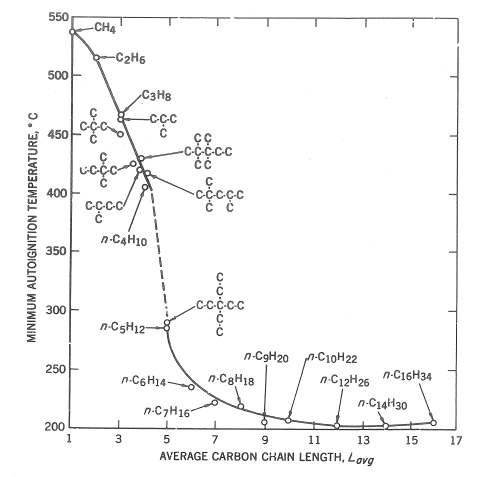
\includegraphics[width=5cm]{zabetakis.PNG}
\caption{AIT as a function of carbon chain length (Zabetakis\textsuperscript{[4]})}
\end{figure}
    Mentioned combustion process is a chain of hundreds of different chemical reactions. The initial reactions heat up the mixture through slow oxidation which incites faster reactions which cause the actual autoignition. The chain could be described with one global equation: \par
              
    \begin{equation*}
    	CH_4 + O_2 = CO_2 + 2 H_2O\\        
    \end{equation*}
    or in case of combustion in air:
    \begin{equation*}
    	CH_4 + 2(O_2+3.76N_2) = CO_2 + 2H_2O + 7.52 N_2 
     \end{equation*}
     
     As shown in the equation, in case of methane-air combustion, for every mole of methane 9.52 moles of air are necessary for stoichiometric combustion.
     
     \subsection{Hydrogene}
     
	The reaction of hydrogene's combustion  in air is as follows:
	 \begin{equation*}
    	H_2 + 0.5(O_2+3.76N_2) = H_2O + 1.88N_2 
     \end{equation*}
     For every one mole of hydrogene 2.38 moles of air are needed.
     
       
    \section{Simulation}
    
    \subsection{Methodology}
    	The influence of initial parameters such as chemical composition and absolute pressure was examined utilizing Cantera environment for chemical kinetics calculations in Python. The simulation is run inside a reactor network including a singular 0-dimensional adiabatic reactor. \par 
        A perfectly homogeneous fuel-air mixture is placed inside at t=0 and its parameters i.e. molar fractions of its components, initial temperature and initial absolute pressure are set. Subsequently, simulation time advances by 600s which according to previous researches is predominantly long enough for auto-ignition to occur. Only one time step was used in order to minimize computing time since autoignition delay time is negligible to this simulation. \par 
        Autoignition is determined to have had occurred if the temperature inside of the reactor is at least 200K higher than the initial. Every set of parameters resulting in an autoignition is stored for later use in graphs. \par
        \newpage
        The following simulations were carried out:
\begin{enumerate}
  \item 60\% methane in air cobustion.
  \item 9.5\% methane in air cobustion (stoichiometric)
  \item 60\% hydrogen in air combustion
  \item 29.5\% hydrogen in air cobustion (stoichiometric)
\end{enumerate}
        The first task of the simulation is to find the autoignition temperature of amixture as a function of absolute pressure changing from 0,5 bar to 35 bar by calculating the AIT every 0.5 bar.\par
        The second task is to examine how the AIT changes with the equivalence ratio. Pressure of one atmosphere was set while the number of moles changes from 0.1 to 10 with a step of 0.1 moles. It was then  converted into equivalence ratios.\par 
        Respecting calculation speed, the autoignition temperature is first approximated within a 50K-wide window. Then, more precise calculations take place within that window in order to determine the AIT down to 0.5K.\par
        In order to obtain smoother plots a pressure and temperature step could be reduced at will, but in this way calculations would last longer respectively.\par
        Calculations were repeated for two different molar ratios of methane and hydrogen in air (60\% and stoichiometric)
     

    \section{Results}
    
    \subsection{AIT as a function of initial pressure}
    
\begin{figure}[h]
\begin{subfigure}{.5\textwidth}
\centering
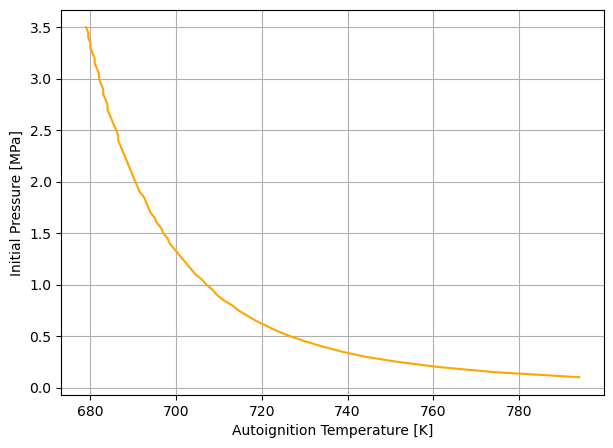
\includegraphics[width=6cm]{1metan60.png}
\caption{60\% methane-air mixture}
\end{subfigure}
\begin{subfigure}{.5\textwidth}
\centering
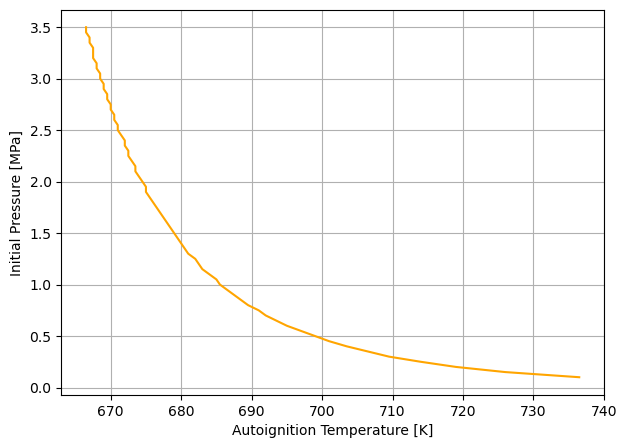
\includegraphics[width=6cm]{1metan9.5.png}
\caption{9.5\% methane-air mixture (stoich.)}
\end{subfigure}
\caption{Autoignition temperature as function of initial pressure in methane-air mixture}
\end{figure}

\begin{figure}[h]
\begin{subfigure}{.5\textwidth}
\centering
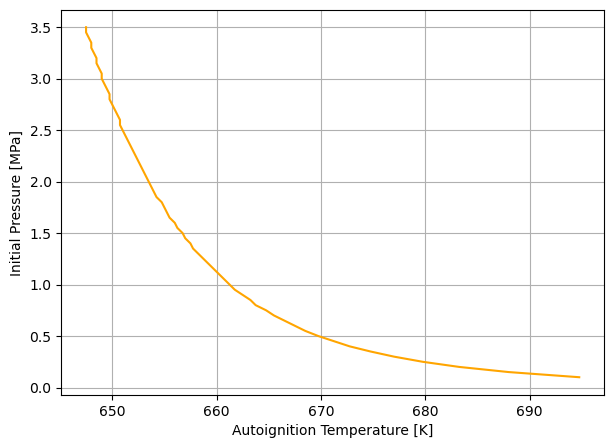
\includegraphics[width=6cm]{1wodor60.png}
\caption{60\% hydrogen-air mixture}
\end{subfigure}
\begin{subfigure}{.5\textwidth}
\centering
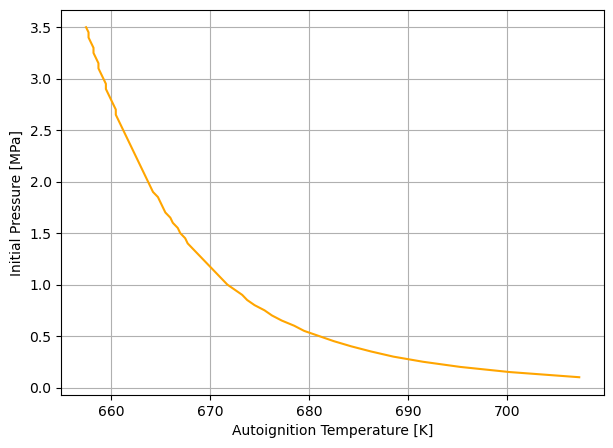
\includegraphics[width=6cm]{1wodor29.5.png}
\caption{29.5\% hydrogene-air mixture (stoich.)}
\end{subfigure}
\caption{Autoignition temperature as function of initial pressure in hydrogen-air mixture}
\end{figure}

	As expected, the relationship between autoignition temperature and initial total pressure of mixture is exponential. As the pressure increases, the temperature drops. The first two plots relate to methane-air mixture in different composition – first one is 60\% and second 9.5\% (stoichiometric). For example, for the initial pressure of 1MPa, from the left plot we observe the AIT of 708K and for the right plot – 686K. It suggests, that in case of methane the richer mixture (\textPhi \ more than one) increases AIT, which is beneficial from the point of view of storing flammable methane.\par
	These findings correspond to the results of Frederik Norman's study\textsuperscript{[3]} presented on the Fig. 4.1.3 

\begin{figure}[h]
\centering
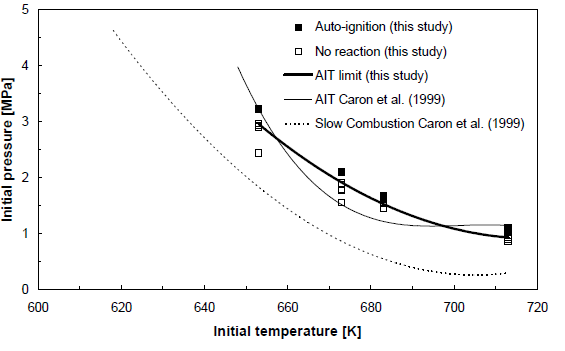
\includegraphics[width=8cm]{norman.PNG}
\caption{Results of Norman's study. Initial pressure vs AIT}
\end{figure}

The study determined that the auto-ignition temperature of 60\% methane-air mixture at pressure od 1MPa is about 715K.\par
	In case of the hydrogen, the AIT is lover comparing to the same molar franctions in methane-air mixture. This means that hydrogen is more dangerous to be stored. From figure 4.1.2 (a) we can see that for the initial pressure of 1MPa the AIT is about 661K, whilst from figure 4.1.2 (b) for the same pressure the AIT stands at 672K. In other words, richer mixture decreases AIT. This informs us, that hydrogen should be stored in lower molar fractions, on the contrary to methane.\par

\subsection{AIT as a function of mixture's composition}

\begin{figure}[h]
\begin{subfigure}{.5\textwidth}
\centering
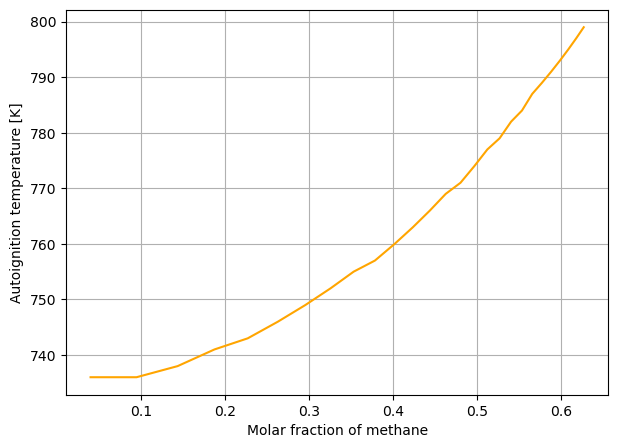
\includegraphics[width=6cm]{2metan.png}
\caption{AIT as a function of molar fraction}
\end{subfigure}
\begin{subfigure}{.5\textwidth}
\centering
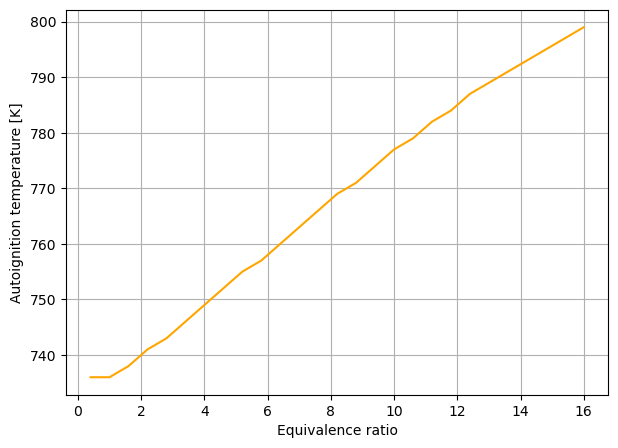
\includegraphics[width=6cm]{3metan.png}
\caption{AIT as a function of equivalence ratio}
\end{subfigure}
\caption{AIT as a function of molar fractions for methane combustion in air}
\end{figure}

\begin{figure}[h]
\begin{subfigure}{.5\textwidth}
\centering
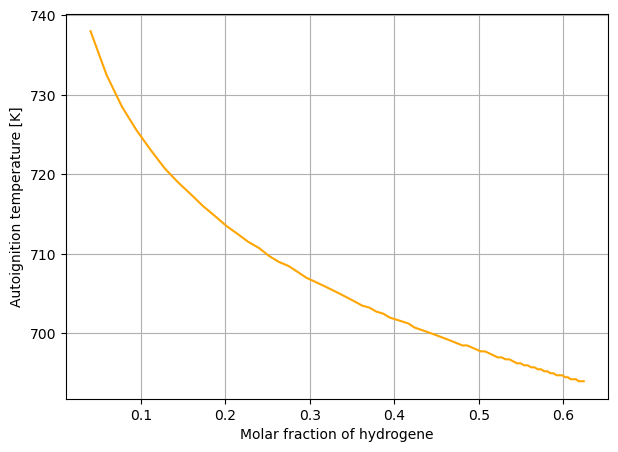
\includegraphics[width=6cm]{2wodor.png}
\caption{AIT as a function of molar fraction}
\end{subfigure}
\begin{subfigure}{.5\textwidth}
\centering
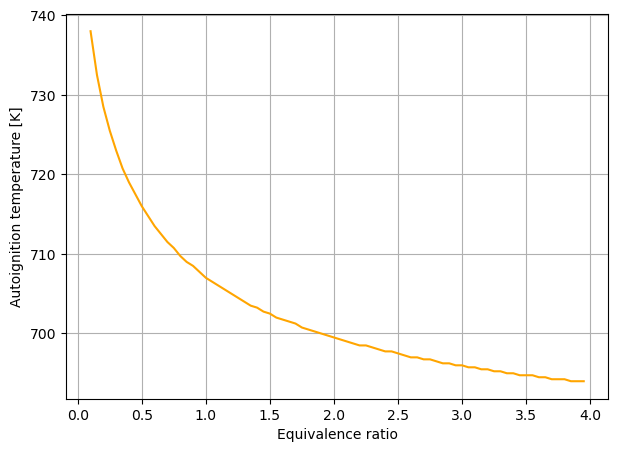
\includegraphics[width=6cm]{3wodor.png}
\caption{AIT as a function of equivalence ratio}
\end{subfigure}
\caption{AIT as a function of molar fractions for hydrogen combustion in air}
\end{figure}
	This simulation confirms the results obtained in chapter 4.1. The growth of molar fraction in methane-air mixture  increases AIT, oppositely to hydrogen-air mixture. The character of the plot 4.2.1 (a) is exponential, but the relation between AIT and equivalence ratio is linear (plot 4.2.1 (b)). \par
	On the other hand, on the example of hydrogen we can notice two exponential correlations. For the hydrogen the AIT is the lowest (around 700K) when equivalence ratio is equal to 4.0. For methane the lowest autoignition temperature is 735K for molar fraction near stoichiometric. 

\section{Conclusions}
   The purpose of this report was to examine the influence of the initial total pressure and mixture composition on the autoignition temperature of two flammable mixtures on the examples of methane and hydrogen.\par
    The results are unambiguous. The pressure of the mixture ought to close to atmospheric in order to avoid auto-ignition. Gaseous methane is more exposed to auto-ignition with a great amount of oxidizer, entirely oppositely to hydrogen.\par
    Knowing about auto-ignition temperature is very important when it comes to storage of flammable gases.

    \section{References}
    
\begin{enumerate}
\item  Cezary Kardas, \textit{Influence of mixture composition and initial pressure on the autoignition temperature of methane-air mixture}, April 2017 \url{https://github.com/cezkardas/MKWS.git}

\item  Nicholas P. Cheremisinoff, Paul Rosenfeld and Anton R. Davletshin \textit{Responsible Care,
A New Strategy for Pollution Prevention and Waste Reduction Through Environment Management}, 2008

\item  Frederik Norman, \textit{Influence of Process Conditions On The Auto-Ignition Temperature of Gas Mixtures}, Katkolieke Universiteit Leuven, Faculteit Ingenieurswetenschappen, June 2008

\item SAFEKINEX, \textit{Report on experimentally determined self-ignition temperature and the ignition delay time, Federal Institute for Materials Research and Testing}, 2002 
\item Anne Felden, \textit{CANTERA Tutorials}, Tutorial 4, CERFACS, November 2015 

\item Zabetakis, M.G., Rurno, A.L. and Jones, \textit{Minimum spontaneous
ignition temperatures of combustibles in air}, Industrial Engineering Chemistry, 1954
2173–2178
\end{enumerate}
    
\end{document}